\chapter*{PARTIE 1 : La genèse d’une nouvelle science}
\addcontentsline{toc}{part}{PARTIE 1 : La genèse d’une nouvelle science}
\markboth{La genèse d’une nouvelle science}{La genèse d’une nouvelle science}
\origpage{57}{043}
Si les deux chapitres liminaires étaient une approche à petits pas, cette première partie constitue un voyage :
\begin{itemize}
\item un voyage dans le temps d’abord : s’ouvrant sur l’antiquité pour s’achever dans les toutes premières années du 20\textsuperscript{e} siècle, elle couvre une période de plus de 2000 ans.
\item un voyage dans l’espace ensuite : le langage étant une faculté universelle, les savants des quatre coins du monde se sont penchés sur cette question. Dans cette partie, on rencontra\ednote{原文 « on rencontra » 为简单过去时；本段是在预告下文，与后面的 « nous verrons »、« nous allons » 一致时，应作 « on rencontrera »。} donc un grand nombre de grammairiens, logiciens, philosophes et linguistes indiens, romains, grecs, anglais, allemands, danois, français, suisses et chinois.
\end{itemize}
Ayant pour but de retracer le cheminement intellectuel qui a permis la naissance de la linguistique moderne, cette partie est structurée en quatre chapitres, comme suit :
\begin{center}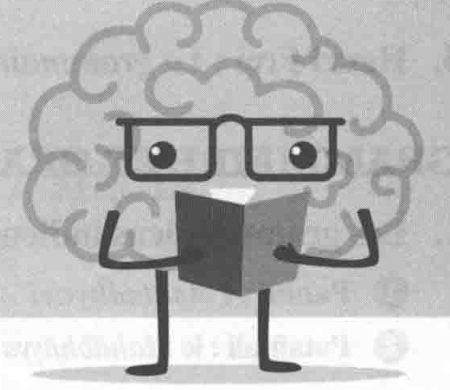
\includegraphics[width=.30\linewidth]{assets/partie1_illustration.png}\end{center}
\minititle{Le chapitre 3}
De la grammaire à la linguistique : quand un art devient science retrace le long processus par lequel la grammaire (\textit{ars grammatica}, en latin) est devenue au fil du temps une véritable science (la linguistique). Dans ce chapitre, nous verrons tout ce que notre linguistique moderne doit à ces véritables précurseurs des études sur le langage qu’ont été les grammairiens de l’antiquité, du Moyen Âge, de la renaissance et de l’époque classique.
\minititle{Le chapitre 4}
Logique et linguistique : les deux sciences du \textit{logos}, est centré autour du concept grec de \textit{logos} qui signifie à la fois « langage » et « raisonnement ». Après une présentation de la logique antique et médiévale, et après avoir mis en évidence les limites existant entre la logique et le langage, nous verrons comment ce \textit{logos} unique s’est scindé pour donner naissance à deux sciences distinctes : une science du raisonnement et une science du langage.
\minititle{Le chapitre 5}
Linguistique comparative : la diversité des langues, nous allons nous intéresser à la grammaire comparative et répondre à la question : comment classer les sept-mille langues que compte notre planète? Antichambre de la linguistique moderne, cette grammaire comparative est née des travaux de savants polyglottes (William Jones, Friedrich Schlegel, Franz Bopp, etc.) dont le mérite est d’avoir décelé, derrière l’apparente diversité des langues, des ressemblances qui permettent de les classer soit sur la base de liens de parenté (famille indoeuropéenne, par exemple), soit sur la base de ressemblances formelles : langues isolantes, agglutinantes, et synthétiques.
\minititle{Le chapitre 6}
Théories du signe : Peirce et Saussure, nous arrivons à l’époque moderne et assistons à la naissance de la sémiologie, sciences des signes\ednote{此处以同位语说明单数名词 « la sémiologie »，应为 « science des signes »。} qui a la particularité d’avoir deux « papas » — l’américain Charles S. Pierce\ednote{原文此处作 « Pierce »，与同句开头及第六章题名中的 « Peirce » 不一致；应为 Charles S. Peirce。} et le suisse Ferdinand de Saussure. Avec la publication posthume de son célèbre \textit{Cours de Linguistique Générale} (1916), Saussure est également considéré, surtout en Europe, comme le fondateur de la linguistique moderne.
